\documentclass[11pt,titlepage]{article}

%Laenderspezifische Einstellungen bzgl. Rechtschreibung, Sonderzeichen und Kodierung
\usepackage[utf8]{inputenc}
\usepackage[english]{babel}
\usepackage[T1]{fontenc}
\usepackage{titlesec}
\usepackage{graphicx}
%\usepackage{subcaption}

\usepackage{listings}
\usepackage{color}
\usepackage{courier}
\definecolor{light-gray}{gray}{0.85}
\lstset{
language=C++,
numbers=left,
breaklines=true,
backgroundcolor=\color{light-gray},
tabsize=2,
basicstyle=\footnotesize\ttfamily,
frame=single,
inputencoding=utf8,
extendedchars=true,
showstringspaces=false,
literate =
	{ä}{{\"a}}1
	{ö}{{\"o}}1
	{ü}{{\"u}}1
	{Ä}{{\"A}}1
	{Ö}{{\"O}}1
	{Ü}{{\"U}}1
	{ß}{{\ss}}1
	{ₙ}{{$_n$}}1
}

\def\ContinueLineNumber{\lstset{firstnumber=last}}
\def\StartLineAt#1{\lstset{firstnumber=#1}}		%\StartLineAt{xxx}	

\usepackage[
	a4paper,
	top = 2cm,
	bottom = 2 cm,
	left = 2cm,
	right = 2cm,
	headheight = 15pt,
	includeheadfoot
	]{geometry}
\usepackage{fancyhdr}
\usepackage{amssymb}
\usepackage{amsmath}
\usepackage[english]{varioref}
\usepackage{hyperref}

\fancypagestyle{fancy}{
	\fancyhead[R]{Page \thepage}
	\fancyhead[L]{\leftmark}
	\renewcommand{\headrulewidth}{1.25pt}

	\fancyfoot[L]{\tiny{Programming 2 - Assignment 3, created: \today}}
	\fancyfoot[R]{\tiny{ Felix Dreßler (k12105003)}}
	\cfoot{}
	\renewcommand{\footrulewidth}{1.25pt}
}

\setlength{\headsep}{10mm}
\setlength{\footskip}{10mm}

\setlength{\parindent}{0mm}
\setlength{\parskip}{1.1ex plus0.25ex minus0.25ex}
\setlength{\tabcolsep}{0.2cm} % for the horizontal padding

\pagestyle{fancy}

\title{Programming 2 - Assignment 3}
\author{Felix Dreßler (k12105003)\\ email \href{mailto:FelixDressler01@gmail.com}{FelixDressler01@gmail.com}}
\date{\today} %Erstellungsdatum

\begin{document}
\maketitle
	\section{Testing the Program}
		\subsection{Testing Code - Main.cpp}
		
		\subsection{testing - output}


	\section{Problems}
	This section will briefly discuss the Problems that have occurred during programming.
		\subsection{virtual functions/Data types}
			Despite the best efforts, there is still a problem with the code. Specifically concerning the \emph{Picture} class. While drawing a picture, the outputted polygons of type \emph{RegularPolygon} do not contain a center point. In the following two sections, the code which was used to narrow the problem down and its output are presented.
			The code contains multiple \emph{cout}s to determine where exactly the problem lies.
			We can see, that while adding polygons to the \emph{LinkedList} of the picture, that holds pointer to polygons, the correct \emph{clone()} function of the respective derived class is called. But when calling the \emph{draw()} function, it always calls the virtual function defined in the \emph{Polygon} class.
			
			This Problem is probably caused by the type that those polygons hold during runtime of the program. Because the \emph{LinkedListPointer} stores just pointer to polygons (\emph{Polygon*}) this could be caused by the declaration of the type of pointer inside there.
			
			The testing of clone and draw, that we have already done suggests, that these functions are created correctly.
			\subsubsection{testing code}	
		
				\lstinputlisting[]{Documentation/Problems/main.cpp}
		
			\subsubsection{output of the testing code}	
	
				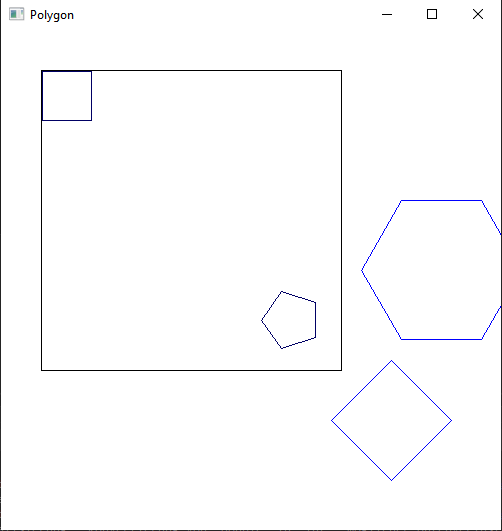
\includegraphics[scale=0.5]{Documentation/Problems/problem.png}
				
				\begin{lstlisting}[numbers=none]
					add p - Polygon
					clone - Polygon
					add q - Regular
					clone - Regular Polygon
					add r - Regular
					clone - Regular Polygon
					add s - Regular
					clone - Regular Polygon
					draw - Polygon
					draw - Polygon
					draw - Polygon
					draw - Polygon
					draw - Polygon
				\end{lstlisting}
	
\newpage
	\section{The Program}
	

		\subsection{The Program - Polygon}
			\subsubsection{Polygon.h}
				\lstinputlisting[]{Assignment3/Project1/Polygon.h}
				
			\subsubsection{Polygon.cpp}
				\lstinputlisting[]{Assignment3/Project1/Polygon.cpp}
		
		\subsection{The Program - Picture}
			\subsubsection{Picture.h}
				\lstinputlisting[]{Assignment3/Project1/Picture.h}
			
			\subsubsection{Picture.cpp}
				\lstinputlisting[]{Assignment3/Project1/Picture.cpp}
		
		\subsection{The Program - Linked Lists}
			\subsubsection{LinkedListArr.h}
				\lstinputlisting[]{Assignment3/Project1/LinkedList.h}
			
			\subsubsection{LinkedListArr.cpp}
				\lstinputlisting[]{Assignment3/Project1/LinkedList.cpp}
			
			\subsubsection{LinkedListPointer.h}
				\lstinputlisting[]{Assignment3/Project1/LinkedListPointer.h}
				
			\subsubsection{LinkedListPointer.cpp}
				\lstinputlisting[]{Assignment3/Project1/LinkedListPointer.cpp}
				

		
	
\end{document}